\documentclass[11pt,twoside]{scrartcl}
%\documentclass[11pt,twoside]{article}

%opening
\newcommand{\lecid}{15-316}
\newcommand{\leccourse}{Software Foundations of Security and Privacy}
\newcommand{\lecdate}{} %e.g. {October 21, 2013}
\newcommand{\lecnum}{8,9}
\newcommand{\lectitle}{Security Automata \& Instrumentation}
\newcommand{\lecturer}{Matt Fredrikson}
\newcommand{\lecurl}{https://15316-cmu.github.io/index}

\usepackage{varwidth}
\usepackage{lecnotes}
\usepackage[irlabel]{bugcatch}

\usepackage{tikz}
\usetikzlibrary{automata,shapes,positioning,matrix,shapes.callouts,decorations.text,patterns,trees,backgrounds}

% \usepackage[bracketinterpret,seqinfers,sidenotecalculus]{logic}
% \newcommand{\I}{\interpretation[const=I]}

% \newcommand{\bebecomes}{\mathrel{::=}}
% \newcommand{\alternative}{~|~}
% \newcommand{\asfml}{F}
% \newcommand{\bsfml}{G}
% \newcommand{\cusfml}{C}
% \def\leftrule{L}%
% \def\rightrule{R}%

\begin{document}

\newcommand{\atrace}{\sigma}%
%% the standard interpretation naming conventions
\newcommand{\stdI}{\dTLint[state=\omega]}%
\newcommand{\Ip}{\dTLint[trace=\atrace]}%
\newcommand{\ws}{\omega}\newcommand{\wt}{\nu}% 

\maketitle
\thispagestyle{empty}

%%%%%%%%%%%%%%%%%%%%%%%%%%%%%%%%%%%%%%%%%%%%%%

\section{Introduction \& Recap}

We began studying safety properties by intuiting that they describe systems where something ``bad'' never happens, and have seen that contracts, assertions, memory safety, and more granular forms of sandboxing are all instances of safety.
But there are certainly other types of bad events that we might want to write policies to enforce against, and aside from finding a way to encode them in programs using assertions, it isn't clear how we would go about doing this.

Today we will generalize what we have learned about enforcing safety by first encoding the bad prefixes using automata, and then monitoring a trace as it evolves though exection.
This style of policy, called \emph{security automata}~\cite{Schneider2000}, is powerful enough to encapsulate all of the safety properties that can possibly be enforced at runtime, and is thus an indespensible tool for ensuring code safety.

\section{Security automata}

To begin developing an intuition for how safety properties can be represented using automata, we return to invariant properties---arguably the simplest type of safety property that we studied.
Suppose that we want to enforce a condition on $x$, e.g.,
\[
0 \le x
\]
In terms of bad prefixes, we could characterize this as any trace containing a state in which $x < 0$.
We could imagine ``watching'' the trace as it develops, and if it ever enters such a state, we would know that safey has been violated.
This type of monitoring can be formalized by constructing a finite automaton, whose states represent the status of our policy, and whose transitions correspond to the current, most-recent state of the program's trace.

In this case, our simple policy has a single status, namely whether $0 \le x$ has remained true so far in the trace.
While we may observe many distinct states as the program executes, the only fact that matters from our perspective is whether this predicate remains true in the current state.
To capture all this, we can draw the following automaton.
\begin{center}
\scalebox{1}{%
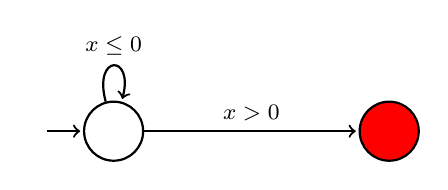
\begin{tikzpicture}
[
  highlight/.style={draw=blue, text=blue},
  shorten >=1pt,
  node distance=2cm,
  on grid,
  auto,
  /tikz/initial text={},
  font=\footnotesize,
  thick
]
 \node[state,thick,initial left,inner sep=1pt,minimum size=0.75cm] (l0) {};
 \node[state,thick,inner sep=1pt,minimum size=0.75cm,fill=red] (l1) [right=3.5cm of l0] {$\errstate$};
 % \node[state,thick,inner sep=1pt,minimum size=0.75cm,fill=red] (l6) [left=3.5cm of l0] {$\errstate$};

  \path[->] 
    (l0) edge [thick,loop above] node [above] {$x \le 0$} (l0)
    (l0) edge [thick] node [above] {$x > 0$} (l1);
\end{tikzpicture}
}
\end{center}
This tells us everything that we need to know to enforce the invariant as we watch the trace unfold.
We begin in a state where the policy has not yet been violated, because the program has not done anything yet.
At each moment before a command is executed, we examine the current state, and match one of the conditions on the transitions to update the status of the policy.
If we ever reach the error state, then we must have seen a bad prefix, and the policy is violated.

Notice that we do not really need to make the error state quite so explicit, and could just as easily leave it implicit.
\begin{center}
\scalebox{1}{%
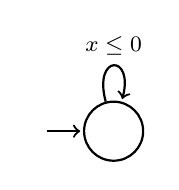
\begin{tikzpicture}
[
  highlight/.style={draw=blue, text=blue},
  shorten >=1pt,
  node distance=2cm,
  on grid,
  auto,
  /tikz/initial text={},
  font=\footnotesize,
  thick
]
 \node[state,thick,initial left,inner sep=1pt,minimum size=0.75cm] (l0) {};
 % \node[state,thick,inner sep=1pt,minimum size=0.75cm,fill=red] (l6) [left=3.5cm of l0] {$\errstate$};

  \path[->] 
    (l0) edge [thick,loop above] node [above] {$x \le 0$} (l0);
\end{tikzpicture}
}
\end{center}
Here, rather than waiting to enter the error state, we merely want to make sure that there always exists some transition with a label that describes the most recent state in the trace.
If we ever see a state that does not satisfy any of the transition labels emanating from the current policy state (i.e., one where $x > 0$), then we conclude that the current prefix must be bad, and the policy is violated.
This is called a \emph{security automaton}~\cite{Schneider2000}, and is the main abstraction that we will use to encode safety in this lecture.

\subsection{A more interesting example.}
As the states comprising traces in our language consist of variable and memory mappings, we have so far been unable to formalize properties that account for the commands that are executed over time.
For example, if our language has the ability to make system calls, such as \psend and \precv from the network and \pread from a local file, we might want to enforce a policy which says that a program should not send data over the network after it has read from local files.
This is indeed a safety property, but to understand it in terms of bad prefixes, we would need to extend the states in our semantics to reflect the commands that are executed.

\paragraph{Accounting for commands.}
Namely, we could formalize states as triples $(\omega_V, \omega_M, \pcderef)$ consisting of variable mappings $\omega_V$, memories $\omega_M$, and ``program counters'' \pcderef.
Unlike $\omega_V$ and $\omega_M$, the \pcderef component is not a mapping, but rather a value ranging over programs.
We could easily extend the semantics of the language to maintain this state, for example:
\[
      \m{\iaccess[\pupdate{\umod{x}{\astrm}}]{\I}}
      =
      \begin{tabular}{l}
      \(\{(\iget[state]{\I},\iget[state]{\It}) \with \omega\llbracket\astrm\rrbracket~\text{defined,}~
      \iget[state]{\It}=\iget[state]{\I}~\text{except}~ \nu_V(x)=\ivaluation{\I}{\astrm},~
      \iget[state]{\It}_\pcderef=\pupdate{\umod{x}{\astrm}}\}\ \cup\) 
      \\
      \(\{(\iget[state]{\I},\errstate) \with \omega\llbracket\astrm\rrbracket~\text{is not defined},~
      \iget[state]{\It}_\pcderef=\pupdate{\umod{x}{\astrm}}\}\)
      \end{tabular}
\]
There are multiple ways that we could update the semantics of compound commands like $\asprg;\bsprg$ and $\pif{\asfml}{\asprg}{\bsprg}$.
The most straightforward would be to leave their semantics unchanged, merely carrying the updates to \pcderef made by the \emph{atomic} commands forward.
In other words, consider the following program.
\[
x := y; \mathtt{Mem}(x) := 0
\]
The traces of this program have three states $\omega_0,\omega_1,\omega_2$.
Because nothing has executed in the initial state, we would assume that \pcderef takes a ``null'' value, e.g., $\varnothing$.
After the first command executes, $\pcderef$ in $\omega_1$ would be $x := y$, and in the final state, $\pcderef = \mathtt{Mem}(x) := 0$.
This would be a consequence of maintaining the usual semantics for sequential composition:
\[
\iaccess[{\alpha};{\beta}]{\I} =
      \{\atrace \compose \varsigma \with \atrace\in\iaccess[\alpha]{\I} \mand \varsigma\in\iaccess[\beta]{\I}\}
\]
In other words, we want \pcderef to point to the most recent command that resulted in a new state, and the commands that cause this are atomic (i.e., variable update, memory update, and $\mathtt{assert}$).

The alternative would be to add a state when the compound command begins executing, so that the way in which the program is composed is reflected in traces.
\[
\iaccess[{\alpha};{\beta}]{\I} =
      \{\omega \compose \atrace \compose \varsigma \with 
      \omega = \atrace_0~\text{except that}~\omega_\pcderef=\alpha;\beta,~\atrace\in\iaccess[\alpha]{\I} \mand \varsigma\in\iaccess[\beta]{\I}\}
\]
This approach might be useful if we need to define safety properties that depend on the composition of commands.
However, the downside is that the updates to the semantics are more extensive, and slightly less intuitive.
For the remainder of the lecture, we will assume that the semantics are updated only to record the execution of atomic commands, and the semantics of compound commands are left unchanged.

\paragraph{No send after read.}
Depicted below is a security automaton for the safety policy ``no send after read''. The states are abstract in the sense that they do not reflect anything about the state of the program or what it is currently doing. Rather, they represent the state at which the policy is currently in. The transitions reflect facts about program state that must be true in order for the automaton to transition. In this case, $\pc$ denotes the current program counter, and $\pcderef$ its contents. So for example $\pcderef \ne \pread$ corresponds to states in which the current instruction pointed to by the program counter is not \pread.
\begin{center}
\scalebox{1.2}{%
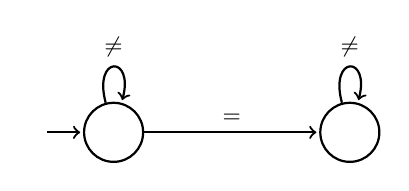
\begin{tikzpicture}
[
  highlight/.style={draw=blue, text=blue},
  shorten >=1pt,
  node distance=2cm,
  on grid,
  auto,
  /tikz/initial text={},
  font=\footnotesize,
  thick
]
 \node[state,thick,initial left,inner sep=1pt,minimum size=0.75cm] (l0) {};
 \node[state,thick,inner sep=1pt,minimum size=0.75cm] (l1) [right=3cm of l0] {};

  \path[->] 
    (l0) edge [thick,loop above] node [above] {$\pcderef \ne \pread$} (l0)
    (l0) edge [thick] node [above] {$\pcderef = \pread$} (l1)
    (l1) edge [thick,loop above] node [above] {$\pcderef \ne \psend$} (l1);
\end{tikzpicture}
}
\end{center}
Notice that as was the case with the invariant policy earlier, the only arrow going out of the rightmost state is a self-loop labeled $\pcderef \ne \psend$. There are no accepting states in a security automaton, and the way to interpret them is that as long as the automaton can transition from some arrow in its current state, then the policy has not been violated. So in this case, if the current policy state were the rightmost one, and the program entered into a state where $\pcderef = \psend$, then there would be no arrow to transition from and the policy would become violated.

Another way to think about it is that there is a ``hidden'' error state which corresponds to the policy being violated. Every node has a transition to the error state on the condition that is the negation of all other outgoing transitions from that state, as shown in the diagram below.
\begin{center}
\scalebox{1}{%
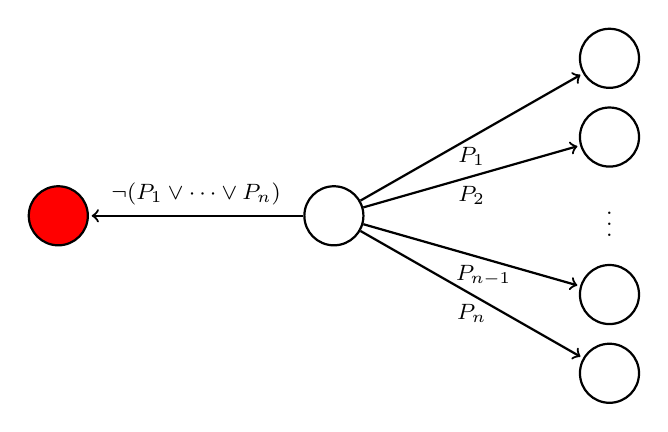
\begin{tikzpicture}
[
  highlight/.style={draw=blue, text=blue},
  shorten >=1pt,
  node distance=2cm,
  on grid,
  auto,
  /tikz/initial text={},
  font=\footnotesize,
  thick
]
 \node[state,thick,inner sep=1pt,minimum size=0.75cm] (l0) {};
 \node[state,thick,inner sep=1pt,minimum size=0.75cm,yshift=2cm] (l1) [right=3.5cm of l0] {};
 \node[state,thick,inner sep=1pt,minimum size=0.75cm] (l2) [below=1cm of l1] {};
 \node[state,thick,inner sep=1pt,minimum size=0.75cm,draw=none] (l3) [right=3.5cm of l0] {\vdots};
 \node[state,thick,inner sep=1pt,minimum size=0.75cm,yshift=-2cm] (l5) [right=3.5cm of l0] {};
 \node[state,thick,inner sep=1pt,minimum size=0.75cm] (l4) [above=1cm of l5] {};
 \node[state,thick,inner sep=1pt,minimum size=0.75cm,fill=red] (l6) [left=3.5cm of l0] {$\errstate$};

  \path[->] 
    (l0) edge [thick] node [below] {$P_1$} (l1)
    (l0) edge [thick] node [below] {$P_2$} (l2)
    (l0) edge [thick] node [below,xshift=1ex] {$P_{n-1}$} (l4)
    (l0) edge [thick] node [below] {$P_{n}$} (l5)
    (l0) edge [thick] node [above] {$\lnot(P_1 \lor \cdots \lor P_n)$} (l6);
\end{tikzpicture}
}
\end{center}
These definitions are equivalent, and we will continue using the convention that does not explicitly list the error state as this will reduce clutter in our diagrams.

\begin{definition}[Security automaton\cite{Schneider2000}]
\label{def:sa}
A security automaton is a nondeterministic state machine that consists of the following components:
\begin{itemize}
\item a countable set $O$ of automaton states,
\item a countable set $O_0 \subseteq O$ of initial states,
\item a countable set $\Sigma$ of transition symbols,
\item a transition relation $\delta \subseteq O \times \powerset{\Sigma} \times O$ between automaton states and sets of transition symbols.
\end{itemize}
We will assume that the transition symbols always correspond to program states, and that sets of program states are represented by formulas that can be evaluated over program states.
Concretely, the set of states corresponding to a formula is comprised of exactly the states that the formula is true in.
Given a sequence of transition symbols (i.e., states) $\sigma = \sigma_0,\sigma_2,\ldots$, we say that the autoamton accepts $\sigma$ if and only if there is a corresponding sequence of states $o = o_0,o_1,\ldots$ such that for each pair $\sigma_{i},\sigma_{i+1}$ in $\sigma$,
\begin{itemize}
\item there is a corresponding pair $o_{i},o_{i+1}$ of states in $o$,
\item and there exists $(o_{i}, P, o_{i+1}) \in \delta$ where $\sigma_i \vDash P$.
\end{itemize}
In other words, a trace is only accepted if there is a corresponding run of the automaton that always follows the transition function.
\end{definition}

Definition~\ref{def:sa} formally defines security automata in terms of a set of states $O$ and transition symbols $\mathcal{S}$. We will generally assume that $\mathcal{S}$ is the set of all program states, so that we can describe program traces as being accepted or not by a security automaton. This also implies that sets of states in the transition relation are defined in terms of formulas on program states, which we have already studied extensively.

\subsection{Taint analysis}

We have seen that information flow cannot be checked by examining single traces in isolation. But this doesn't mean that they can't be \emph{approximated} in some useful sense by safety properties. One approach for approximating information flow that has been used widely for certain applications is called \emph{taint analysis}~\cite{Schwartz2010}. 

Conceptually, taint analysis enforces a safety property that tracks the portions of program state that have been ``tainted'' by some identified source. The policy maintains state that contains a bit for each variable and memory cell used by the target program. A subset of the variables and memory cells are distinguished as taint ``sources'', and a different subset as the ``sinks''. Then as the program executes, the policy state is updated to reflect the flow of tainted information through the state. If any of the state identified as a sink becomes tainted, then the policy is violated.

\paragraph{Security automaton.}
Taint analysis can be formalized and enforced as a security automaton. We show how by defining the states, initial states, transition symbols, and transition relation. To keep things simple while illustrating the main ideas, we will assume that the language has only variables and no memory state or operations.
\begin{itemize}
\item The states of the automaton correspond to the set of all \emph{taint mappings} $\taint$ from program variables to $\{0,1\}$. Intuitively, if the policy is in a state where $\taint(x) = 1$, then $x$ is currently tainted, and if $\taint(x) = 0$ then it is not.

\item The initial states are all mappings $T$ where $T(x) = 1$ for each identified source variable and $T(y) = 0$ for all non-source variables.

\item The transition symbols are program instructions $\pupdate{\pumod{x}{\astrm}}$, $\passert{\ivr}$, $\pifjump{\ivr}{\astrm}$.

\item The transition relation is defined to \emph{propagate} the taintedness of an expression on the right-hand side of an assignment to the variable on its left-hand side. If $\taint$ is a taint mapping, then we use the following rules to determine whether an expression is tainted.
\begin{center}
\begin{calculus}
\cinferenceRule[var|Var]{Var}{%
\linferenceRule[sequent]
  {\taint(x) = 1}
  {\lsequent{\taint}{x}}
}{}%
\end{calculus}
\quad
\begin{calculus}
\cinferenceRule[opl|OpL]{OpL}{%
\linferenceRule[sequent]
  {\lsequent{\taint}{\astrm}}
  {\lsequent{\taint}{\astrm \cdot \bstrm}}
}{}%
\end{calculus}
\quad
\begin{calculus}
\cinferenceRule[opl|OpR]{OpR}{%
\linferenceRule[sequent]
  {\lsequent{\taint}{\bstrm}}
  {\lsequent{\taint}{\astrm \cdot \bstrm}}
}{}%
\end{calculus}
\end{center}
Then for every assignment instruction $\pumod{x}{\astrm}$ where $x$ is not a sink variable, and pair of states $\taint_1, \taint_2$ where $\lsequent{\taint_1}{\astrm}$ and $\taint_2(x) = 1$, the corresponding edge $(\taint_1, \pumod{x}{\astrm}, \taint_2)$ is in the transition relation. Additionally, for every pair of states $\taint_1, \taint_2$ where $\taint_1 \not\vdash \astrm$ and $\taint_2(x) = 0$, $(\taint_1, \pumod{x}{\astrm}, \taint_2)$ is in the relation. Finally, for every other instruction $\asprg$ that is not an assignment and every state $\taint$, $(\taint, \asprg, \taint)$ is in the transition relation.
\end{itemize}
Let's see how this works for a simple program with variables $x, y,$ and $z$. Suppose that $x$ is a taint source, and $z$ is the sink:
\begin{equation}
\begin{array}{ll}
\mathtt{1:} & z := 0 \\
\mathtt{2:} & y := x \\
\mathtt{3:} & z := y
\end{array}
\end{equation}
The automaton will have eight states, as there are $2^3 = 8$ mappings from the three variables to $\{0,1\}$. We will use a shorthand to denote states that gives the value of the mapping on each variable $x,y,z$ in order. So the initial state maps $x$ to 1, and $y,z$ to 0 and is denoted \verb'[100]'. 

We will only consider edges corresponding to instructions in the program, so the initial state has three possible outgoing edges. On executing either $z := 0$ or $z := y$, none of the taint state changes so we would remain in the initial state. On executing $y := x$ however, the mapping for $y$ changes to 1 because $\lsequent{\mathtt{[100]}}{x}$. So the automaton can transition to \verb'[110]'.
\begin{center}
\scalebox{1.2}{%
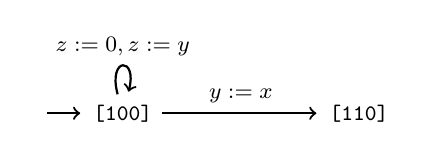
\begin{tikzpicture}
[
  highlight/.style={draw=blue, text=blue},
  shorten >=1pt,
  node distance=2cm,
  on grid,
  auto,
  /tikz/initial text={},
  font=\footnotesize,
  thick
]
 \node[rectangle,thick,initial left,draw=none] (l0) {\texttt{[100]}};
 \node[rectangle,thick,draw=none] (l1) [right=3cm of l0] {\texttt{[110]}};

  \path[->] 
    (l0) edge [thick,loop above] node [above] {$z := 0, z := y$} (l0)
    (l0) edge [thick] node [above] {$y := x$} (l1);
\end{tikzpicture}
}
\end{center}
From state \verb'[110]', executing $z := 0$ or $y := x$ leaves the taint mapping the same, but executing $z := y$ would result in \verb'[111]'. However, $z$ is a sink variable so entering this state would be a policy violation, and we leave the edge out.
\begin{center}
\scalebox{1.2}{%
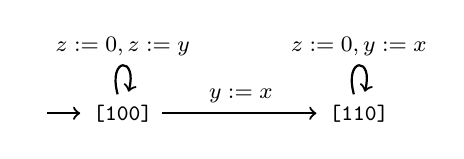
\begin{tikzpicture}
[
  highlight/.style={draw=blue, text=blue},
  shorten >=1pt,
  node distance=2cm,
  on grid,
  auto,
  /tikz/initial text={},
  font=\footnotesize,
  thick
]
 \node[rectangle,thick,initial left,draw=none] (l0) {\texttt{[100]}};
 \node[rectangle,thick,draw=none] (l1) [right=3cm of l0] {\texttt{[110]}};

  \path[->] 
    (l0) edge [thick,loop above] node [above] {$z := 0, z := y$} (l0)
    (l0) edge [thick] node [above] {$y := x$} (l1)
    (l1) edge [thick,loop above] node [above] {$z := 0, y := x$} (l1);
\end{tikzpicture}
}
\end{center}
The full automaton has additional states and transitions. For example, if the taint mapping were \verb'[010]', then executing $y := x$ would transition to \verb'[000]', whereas executing $z := 0$ would stay in the same state. Moreover, executing any instruction in \verb'[000]' stays in that state, so we would add this to the automaton.
\begin{center}
\scalebox{1.2}{%
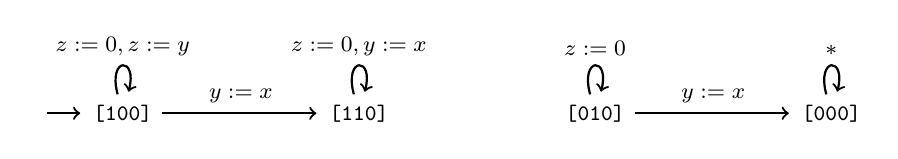
\begin{tikzpicture}
[
  highlight/.style={draw=blue, text=blue},
  shorten >=1pt,
  node distance=2cm,
  on grid,
  auto,
  /tikz/initial text={},
  font=\footnotesize,
  thick
]
 \node[rectangle,thick,initial left,draw=none] (l0) {\texttt{[100]}};
 \node[rectangle,thick,draw=none] (l1) [right=3cm of l0] {\texttt{[110]}};
 \node[rectangle,thick,draw=none] (l2) [right=3cm of l1] {\texttt{[010]}};
 \node[rectangle,thick,draw=none] (l3) [right=3cm of l2] {\texttt{[000]}};

  \path[->] 
    (l0) edge [thick,loop above] node [above] {$z := 0, z := y$} (l0)
    (l0) edge [thick] node [above] {$y := x$} (l1)
    (l1) edge [thick,loop above] node [above] {$z := 0, y := x$} (l1)
    (l2) edge [thick] node [above] {$y := x$} (l3)
    (l2) edge [thick,loop above] node [above] {$z := 0$} (l2)
    (l3) edge [thick,loop above] node [above] {$\mathtt{*}$} (l3);
\end{tikzpicture}
}
\end{center}
But these states are not reachable from the initial state of the SA, so we can leave them out and stop here.

\paragraph{Implicit flows.} So far taint analysis seems to do what we want in terms of tracking information flow as the program executes. So why did we say that it is an approximation of information flow, and moreover, why doesn't this contradict our thought experiment from earlier?

Recall that the program $\asprg_1$ in (\ref{eq:flowexp}) flowed information from $x$ to $y$, effectively computing $y = (1 - x)$. But it did not compute this using an assignment with $x$ on the right hand side, and rather with a conditional statement and constant assignments in either branch. This is known as an \emph{implicit flow} because the information moves from $x$ to $y$ indirectly by the choice of which program to execute within the conditional, rather than explicitly via an assignment statement.

The taint analysis policy that we described doesn't deal with implicit flows because it only propagates taintedness through explicit assignments. In this way taint analysis \emph{underapproximates} information flow. Whenever taint analysis deems that information has flowed from a source to a sink, then an information flow exists in the program. But if it fails to identify a flow, then we can't conclude that there isn't one in the program because there could yet be an implicit flow.

Can we change the security automaton policy to account for implicit flows? Suppose that we added an additional mapping to the policy state, intuitively corresponding to whether the program counter is tainted. We'll denote this $\taint(\pc)$, and we want to make sure that it is set to 1 whenever a conditional statement on a tainted expression is executed. So for example, if $x$ is a source in program (\ref{eq:implicit1}) below, then the policy will be in a state where $\taint(\pc)=1$ after executing the instruction at \keywordfont{1}.
\begin{equation}
\label{eq:implicit1}
\begin{array}{ll}
\mathtt{1:} & \pifjump{x \ne 0}{4} \\
\mathtt{2:} & y := 0 \\
\mathtt{3:} & \pifjump{\mathtt{true}}{5} \\
\mathtt{4:} & y := 1 \\
\mathtt{5:} & \ldots
\end{array}
\end{equation}
Then we can adapt the policy so that whenever $\taint(\pc) = 1$ in the current state, the target of \emph{any} assignment will become tainted. In (\ref{eq:implicit1}), this will ensure that $y$ is tainted after the conditional at \keywordfont{1}, and thus reflect the fact that there is an information flow from $x$ to $y$ in the program.

But now consider what happens if we add another instruction, as in (\ref{eq:implicit2}).
\begin{equation}
\label{eq:implicit2}
\begin{array}{ll}
\mathtt{1:} & \pifjump{x \ne 0}{3} \\
\mathtt{2:} & y := 0 \\
\mathtt{3:} & \pifjump{\mathtt{true}}{5} \\
\mathtt{4:} & y := 1 \\
\mathtt{5:} & z := 0
\end{array}
\end{equation}
Now under the current policy, $z$ will become tainted because it is executed after the tainted conditional. But there is clearly no flow of information from $x$ to $z$, so the taint mapping no longer reflects the actual flows in the program. Perhaps we could refine the policy further, by un-tainting the program counter once control returns to instructions that are in no way conditional on tainted data. In (\ref{eq:implicit2}), this is true for the assignment to $z$ at instruction \keywordfont{5} because it is executed regardless of the condition at \keywordfont{1}.

But how do we identify instructions that aren't conditional on tainted data in general? It was easy in this program, but things could get much more complicated as shown in (\ref{eq:implicit3}).
\begin{equation}
\label{eq:implicit3}
\begin{array}{ll}
\mathtt{1:} & \pifjump{x \ne 0}{6} \\
\mathtt{2:} & y := 0 \\
\mathtt{3:} & \pifjump{\precv\mathtt{()} \ne 0}{7} \\
\mathtt{4:} & \pifjump{\mathtt{true}}{6} \\
\mathtt{5:} & y := 1 \\
\mathtt{6:} & z := 0 \\
\mathtt{7:} & \ldots
\end{array}
\end{equation}
Now in order to tell whether to untaint the program counter before executing instruction 6, we need to predict the outcome of a network read. This policy has gotten significantly more complicated, and keep in mind that we need to do all of these calculations at runtime, which may impose considerable overhead on the target program.

Finally, even if we could solve this problem, tracking taint across implicit flows still may not accurately reflect a program's information flows. Consider the program in (\ref{eq:implicit4}) below.
\begin{equation}
\label{eq:implicit4}
\begin{array}{ll}
\mathtt{1:} & \pifjump{x \ne 0}{3} \\
\mathtt{2:} & y := 0 \\
\mathtt{3:} & \pifjump{\mathtt{true}}{5} \\
\mathtt{4:} & y := \mathtt{complicated\_function()} \\
\mathtt{5:} & \ldots
\end{array}
\end{equation}
It may turn out that $\mathtt{complicated\_function()}$ always returns 0, so that $y$ always takes the same value after the conditional regardless of what $x$ is. In this case, there is no real flow of information from $x$ to $y$. But our security automaton policy can't reason this way, because it would require considering a different trace from the one that was actually executed. Even if it could, it would need to reason about the behavior of an arbitrarily complicated, possibly non-terminating function, which is clearly not possible.

\subsection{Enforcing security automata policies}

The primary means of enforcing policies defined using security automata is with a \emph{reference monitor} (RM). The RM is a mechanism that examines the program as it executes, using information about the current and past states to decide whether the policy has been violated. This is done according to Definition~\ref{def:sae}, and was sketched out at the beginning of this section.

\begin{definition}[Security automaton enforcement]
\label{def:sae}
Let $O_c$ be the current set of states that the security automaton is in. Then for each step that the program is about to take resulting in new program state $\omega$, the reference monitor does one of two things.
\begin{enumerate}
\item For each state $o \in O_c$ that the automaton can transition from, the states $\delta(o,P,o')$ for all transition edges where $\omega \vDash P$ are added to the new automaton states.
\item If the automaton cannot transition from any of its current states, then the program is not allowed to enter state $\omega$ and the reference monitor takes remedial action.
\end{enumerate}
\end{definition}

As long as the policy is not violated, then the RM allows the program to continue executing as it otherwise would. If the policy is violated, then the RM intervenes on the program execution to take some remedial action. This could mean simply aborting the execution, or something less drastic that prevents harm in other ways.

\paragraph{Necessary assumptions.} As pointed out by Schneider in his seminal work on security automata~\cite{Schneider2000}, there are several assumptions that one must make in order to enforce these policies effectively with a reference monitor. First, the reference monitor needs to simulate the execution of the automaton as the program runs, so it must keep track of which state the policy is in on the actual hardware running the program. This means that the automaton cannot require an unbounded amount of memory, so automata that have an infinite number of states are not in general enforceable.

Second, the RM must be able to prevent the program from entering a state that would result in a policy violation. This is called \emph{target control}, and is a more subtle issue that it may at first seem. Take for example the policy of ``real-time'' availability, which states that a principal should not be denied a resource for more than $n$ real-time seconds. How could a reference monitor enforce this policy? It might try to predict the amount of time that it takes to remediate a trace that is about to violate the policy, and take action earlier than necessary to prevent the violation. But how does it know that the policy would have actually been violated in this case? Unless the reference monitor can literally stop time, this is not an enforceable policy.

Third, the program under enforcement must not be able to intervene directly on the state of the reference monitor. This is called \emph{enforcement mechanism integrity}, and is crucial for ensuring that the policy defined by the automaton is the one that is actually enforced on the target program. We dealt with an instance of this issue earlier in the lecture, when we used control flow integrity to make sure that inlined safety checks weren't bypassed by indirect jumps. But now that the policy itself has state, the enforcement mechansim must also guarantee that the target program does not make changes to that state or influence it in any way that doesn't follow the automaton transitions.

\paragraph{Inline SA enforcement.} One approach to implementing security automata enforcement uses inlined checks to update and maintain state set aside to simulate the automaton. If we assume that formulas on SA transitions are formulas over program states, and there are $N$ security automata states, then we can set aside a region of $N$ memory cells at addresses $a_{\textit{sa}}$ through $a_{\textit{sa}}+N$ to hold the current state of the automaton. If $\pderef{a_{\textit{sa}}+i}$ is non-zero, then we assume that the automaton has entered into state $i$, and otherwise not.

Next we need to implement the transition function, updating the contents of $\pderef{a_{\textit{sa}}} - \pderef{a_{\textit{sa}}+N}$ to simulate the automaton. Suppose that the automaton has an edge from states $i$ to $j$ labeled with formula $\ausfml$. Then for each instruction in the program we compute the verification condition of (\ref{eq:savc}).
\begin{equation}
\label{eq:savc}
\dbox{\asprg}{\lnot\ausfml}
\end{equation}
If (\ref{eq:savc}) is valid before executing $\asprg$, then it means that all traces after executing $\asprg$ will satisfy $\lnot\ausfml$. On the other hand, if it is not valid, then at least one trace of $\asprg$ may satisfy $\ausfml$. This means that we need to insert a check whenever Eq~\ref{eq:savc} is not valid.

What check do we insert? At runtime, we will be in a particular state $\omega$. We want to know if after executing $\asprg$, $\ausfml$ will be true, and if it is, then update the state of the automaton. We can accomplish this by simply checking that $\omega \models \dbox{\asprg}{\ausfml}$. Of course, we will want to use axioms to remove the box modality so that the check is actually in terms of arithmetic, and can be easily evaluated.

So we insert instrumentation immediately before $\asprg$ that checks $\pderef{a_{\textit{sa}}+i} \ne 0 \land \dbox{\asprg}{\ausfml}$, and if it is true then sets $\pderef{a_{\textit{sa}+j}}$ to a non-zero value. Then for each state $i$ in the SA, we compute similar checks for transition to the ``error state''. If $i$ has outgoing edges labeled $P_1, \ldots, P_n$, we insert a check for:
\begin{equation}
\pderef{a_{\textit{sa}}+i} \ne 0 \land \dbox{\asprg}{\lnot(P_1 \lor \cdots \lor P_n)}
\end{equation}
If this check passes, it means that the automaton cannot transition from state $i$. If this holds for every state in the automaton, then the instrumentation aborts execution.

The instrumentation described so far only addresses updates to the SA state. We must also take steps to ensure the integrity of the inlined mechanism, and there are two sources of vulnerability.
\begin{itemize}
\item The contents of $\pderef{a_{\textit{sa}}} - \pderef{a_{\textit{sa}}+N}$ must not be modified by any part of the program except the inserted instrumentation. Applying software fault isolation to the untrusted instructions can ensure that this aspect of integrity holds.
\item The inserted instrumentation could be subverted by indirect control flow. Enforcing CFI on the untrusted code using the original control flow graph ensures that this will not happen.
\end{itemize}
This is sufficient to implement a basic inlined security automaton enforcement mechanism. However, it may impose a severe performance overhead due to all the safety checks.

\section{Dynamic instrumentation}
We have been discussing policy enforcement in a somewhat idealized model, where we assume that programs are given to us as source code in a simple language with few instructions. In the ``real world'' this is not usually the case, and we may be forced to deal with large untrusted programs given to us to execute at runtime, and possibly without source code. So we must find a way to enforce policies on bytecode, and presumably fast lest we introduce unacceptable latency into the system.

Suppose that we wish to implement the inline security automata enforcement scheme from the previous section by changing the instructions throughout the program prior to running it. This seems like a reasonable approach, because the scheme just requires that we check verification conditions on each instruction and replace them when necessary. All that we need to assume is the ability to identify instructions, and compute verification conditions.

\subsection{Challenges for static instrumentation}
But bytecode programs on modern architectures like x86 and AMD64/Intel 64 are extremely difficult to reason about statically, and it may not even be possible to identify which instructions the program will end up executing. One practical issue is the fact that programs can generate new instructions by writing to memory, and then use an indirect jump to begin executing the newly-written code. This can be mitigated by the operating system with a \emph{Write XOR Execute} policy, which ensures that any page of memory may be either writeable or executable, but not both. This is effective, but makes some functionality extremely difficult to implement such as language interpreters that do on-the-fly compilation and optimization.

Even with Write XOR Execute, the presence of indirect control flow and variable-length instruction encoding makes it impossible to tell which instructions will actually be executed. The program can do an arbitrarily complicated computation to derive a target address in existing code, so that the static analysis is unable to determine where execution will resume after a jump. If the target address is in the middle of an existing instruction, it may result in a completely different program being executed. Consider the following example, taken from \cite{Hovav07}.
\begin{equation}
\label{eq:bytecode1}
\begin{array}{lcl}
\mathit{Bytecode} & & \mathit{Instruction} \\
\hline
\verb'f7 c7 07 00 00 00' & & \verb'test $0x00000007, %edi' \\
\verb'0f 95 45 c3' & & \verb'setnzb -61(%ebp)'
\end{array}
\end{equation}
This code is taken from the entry point of an encryption routine in the GNU C library, often referred to as simply libc. If execution begins one byte after the entry point of (\ref{eq:bytecode1}), a completely different program is executed.
\begin{equation}
\label{eq:bytecode2}
\begin{array}{lcl}
\mathit{Bytecode} & & \mathit{Instruction} \\
\hline
\verb'c7 07 00 00 00 0f' & & \verb'movl $0x0f000000, (%edi)' \\
\verb'95' & & \verb'xchg %ebp, %eax' \\
\verb'45' & & \verb'inc %ebp' \\
\verb'c3' & & \verb'ret'
\end{array}
\end{equation}
Importantly this implies that given a sequence of bytecodes, there are numerous possible programs that could end up being executed depending on which addresses are targeted by indirect jumps. In order to instrument the right one, a static analysis needs to determine what these addresses will be, and this is an undecidable problem in general. Moreover, it could be that information not available statically, such as network packets, are used in part to compute target addresses, adding yet another very plausible complication for static instrumentation in this setting.

\subsection{Instrumenting with just-in-time compilation}
Perhaps a better approach given these challenges is to delay ``code discovery'' until the program is actually running. This is helpful for many reasons.
\begin{itemize}
\item If the program generated instructions in memory and transferred control to them, we no longer need to infer what those instructions will be. We can simply wait until the program has already written them, and instrument them immediately before the control transfer.
\item If a program executes an indirect jump, we do not need to predict what the target address will be. We simply wait until immediately before the jump is executed, at which point the target address will be stored in memory or a register, and begin instrumenting the target of the jump.
\item Some other cases that we have not discussed are handled similarly, such as libraries that are loaded after the program begins executing. In each such case, the instrumentation is delayed until immediately before the instructions in question begin executing, at which point all of the necessary information is available.
\end{itemize}
The obvious drawback to this approach is the fact that we need to examine the execution as it unfolds, rewriting instructions whenever necessary as dictated by the policy.

\paragraph{Just-in-time compilation.} A successful and widely-deployed approach to mitigate the performance penalty imposed by such a scheme is called \emph{just-in-time (JIT) compilation}~\cite{Aycock2003}. The key insight behind JIT compilation is to increase the granularity at which the instrumenter examines code at runtime, looking at ``chunks'' of instructions rather than individual ones. 

Increasing the granularity in this way allows the instrumenter to compile instruction chunks, with their instrumentation included, on the fly into optimized code that is then executed directly. Further performance enhancements can then be layered on top of this basic approach, such caching previously-compiled chunks to save redundant work, as well as more aggressive optimizations to sequences of chunks that end up being executed more often.

The question then becomes what constitutes a chunk. Larger chunks will generally create more opportunities for optimization, and because more of the instructions are dealt with each time, require fewer (expensive) calls to the compiler. However, this tendency is limited by the fact that if a chunk crosses an indirect control flow instruction, then we run into exactly the same problems we are trying to avoid with dynamic instrumentation in the first place. Even if our chunks cross direct, predictable control flow branches, then we run the risk of doing unnecessary compilation and instrumentation by processing multiple branches when the execution will only end up following one of them.

The typical approach is to use \emph{basic blocks} as chunks. A basic block is a contiguous sequence of instructions that ends in a control flow transfer instruction (e.g., \verb'jmp', \verb'ret', \verb'call', \ldots). For example, the sequence of instructions in (\ref{eq:bytecode2}) is a basic block because it ends with a \verb'ret' instruction, which transfers control to the instruction pointed to by the return address on the stack. On the other hand, (\ref{eq:bytecode1}) is not a basic block because it does not end in such an instruction.

Using basic blocks as chunks, the instrumenter will begin scanning a sequence of bytecodes until it reaches a control transfer instruction. It will then instrument each of the instructions in the basic block as prescribed by the policy, compile the resulting instructions, and execute them. However, it must ensure that it regains control when the basic block is finished executing. It then begins scanning instructions again at the bytecodes pointed to by the instruction pointer, repeating the process all over again. In this way we can be sure that exactly the code that is executed is instrumented according to the policy.
\bibliographystyle{plain}
\bibliography{bibliography}
\end{document}